\documentclass{article}
\usepackage{graphicx} % Required for inserting images
\usepackage{float}
\usepackage[T1]{fontenc}
\usepackage{amsmath}
\usepackage[margin=1in]{geometry}
\usepackage{booktabs}
\usepackage{tabularx}
\usepackage[hidelinks]{hyperref}

\title{FOMC and CPI days in the stress-sized put book}
\author{Diagnostic \textperiodcentered{} L/S Gamma Desk, QUANTT}
\date{2026-11-02}

\begin{document}

\maketitle

\textbf{Question:} Does the always-on, stress-sized 25-delta put book earn differently over FOMC statements and CPI releases than on other days, and is that enough to justify a pre-registered card (for example, skipping entries before CPI or adding size into FOMC)?

\textbf{Method:}

\begin{itemize}

\item \textbf{Runs:} registered runs only; no new trials. The 2026-10-22 \texttt{hedged} book at 1x and 2x spreads, with the one-contract \texttt{always25} book (2026-10-17) at 1x as context. Development window only, 2014-06-02 to 2024-12-31.

\item \textbf{Intervals:} each run's equity is marked once a day at 10:15 ET, so P\&L is measured from one 10:15 mark to the next, as in the 2026-10-31 weekend check. A close-to-close split isn't possible from these runs.

\item \textbf{Interval types:}

\begin{itemize}

\item \textbf{FOMC statement:} the interval containing the 14:00 ET statement, from the statement day's 10:15 mark to the next morning's. All scheduled statements in the window were at 2:00 p.m.

\item \textbf{Day before statement:} the interval ending at 10:15 on statement day.

\item \textbf{CPI release:} the interval containing the 08:30 ET release, from the prior day's 10:15 to the release day's 10:15.

\item \textbf{Other:} everything else.

\item An interval that holds two events counts in both types: 3 FOMC intervals also hold a CPI release, and 9 pre-statement intervals do.

\end{itemize}

\item \textbf{Measures:}

\begin{itemize}

\item book P\&L per interval, in dollars, net of costs;

\item for \texttt{hedged} 1x, P\&L per contract held at the start of the interval, since the book's size varies from 8 to 100 contracts.

\end{itemize}

\item \textbf{The March 2020 window:} the ``ex 19 Feb-30 Apr 2020'' rows drop that window. No scheduled statement fell inside it, because the 17-18 March meeting was cancelled.

\item \textbf{Dates:}

\begin{itemize}

\item 84 scheduled FOMC statements and 127 CPI releases, each checked against the official calendars (see Sources).

\item Aggregates only: no per-trade rows, strikes or prices.

\end{itemize}

\end{itemize}

\section{Short answer}

\begin{itemize}

\item \textbf{FOMC:} the interval across the statement earned more than other days.

\begin{itemize}

\item The \texttt{hedged} book made \$171 per interval against \$49 on other days, with t = 2.0 for the FOMC mean alone. Per contract, it made \$8.1 against \$0.9.

\item The excess holds in both halves and at both spreads.

\item But against the other days, the difference is not significant: Welch t = 1.3 in dollars and 1.8 per contract.

\item The book already holds a put through 83 of the 84 statements.

\end{itemize}

\item \textbf{CPI release intervals lost slightly:} \ensuremath{-}\$59 per interval, t = \ensuremath{-}0.7.

\begin{itemize}

\item The loss comes from 2020-2024, and 2022 alone is \ensuremath{-}\$9.4k of the \ensuremath{-}\$7.4k total.

\item 2014-2019 was flat.

\end{itemize}

\item \textbf{Neither result justifies a card on its own.}

\begin{itemize}

\item \textbf{``Skip entry before CPI'' can't be tested:} the book opened a put on the day before a CPI release only once in 182 entries.

\item \textbf{``Hold through FOMC''} is what the book already does.

\item The only testable version is \textbf{adding size into the statement.} On this evidence the per-contract excess, about \$7, has to cover an extra round trip: the spread plus \$1.30 of commission per contract. This note didn't check the spread model's cost for that trade.

\end{itemize}

\end{itemize}

\section{Results: hedged book, 1x}

\begin{center}\small
\begin{tabularx}{\linewidth}{>{\raggedright\arraybackslash}X >{\raggedright\arraybackslash}X l l l l}
\toprule
\textbf{Interval} & \textbf{Period} & \textbf{Intervals} & \textbf{Sum} & \textbf{Mean} & \textbf{t (mean)} \\
\midrule
FOMC statement & all & 84 & +\$14,331 & +\$171 & 2.01 \\
FOMC statement & 2014-2019 & 45 & +\$6,229 & +\$138 & 1.40 \\
FOMC statement & 2020-2024 & 39 & +\$8,102 & +\$208 & 1.45 \\
Day before statement & all & 80 & +\$2,520 & +\$32 & 0.76 \\
Day before statement & 2014-2019 & 43 & +\$2,889 & +\$67 & 1.97 \\
Day before statement & 2020-2024 & 37 & \ensuremath{-}\$368 & \ensuremath{-}\$10 & \ensuremath{-}0.12 \\
CPI release & all & 127 & \ensuremath{-}\$7,441 & \ensuremath{-}\$59 & \ensuremath{-}0.70 \\
CPI release & 2014-2019 & 67 & +\$1,252 & +\$19 & 0.20 \\
CPI release & 2020-2024 & 60 & \ensuremath{-}\$8,693 & \ensuremath{-}\$145 & \ensuremath{-}1.02 \\
CPI release & all ex 19 Feb-30 Apr 2020 & 125 & \ensuremath{-}\$6,378 & \ensuremath{-}\$51 & \ensuremath{-}0.61 \\
Other & all & 2,296 & +\$112,816 & +\$49 & 1.56 \\
Other & all ex 19 Feb-30 Apr 2020 & 2,250 & +\$89,845 & +\$40 & 2.44 \\
\bottomrule
\end{tabularx}
\end{center}

The FOMC rows don't change without the March 2020 window, because no scheduled statement fell in it. The pre-statement rows lose one interval: +\$2,777 over 79, mean +\$35.

\subsection{Difference from other days, and the other books}

\begin{center}\small
\begin{tabularx}{\linewidth}{>{\raggedright\arraybackslash}X >{\raggedright\arraybackslash}X l >{\raggedright\arraybackslash}X l}
\toprule
\textbf{Book /\allowbreak{} measure} & \textbf{FOMC: mean vs other} & \textbf{Welch t} & \textbf{CPI: mean vs other} & \textbf{Welch t} \\
\midrule
\texttt{hedged} 1x, \$ per interval & +\$171 vs +\$49 & 1.34 & \ensuremath{-}\$59 vs +\$49 & \ensuremath{-}1.21 \\
\texttt{hedged} 1x, \$ per contract & +\$8.1 vs +\$0.9 & 1.83 & \ensuremath{-}\$3.5 vs +\$0.9 & \ensuremath{-}1.10 \\
\texttt{hedged} 2x, \$ per interval & +\$161 vs +\$41 &  & \ensuremath{-}\$65 vs +\$41 &  \\
\texttt{always25} 1x (1 contract) & +\$5.8 vs +\$0.5 &  & \ensuremath{-}\$3.8 vs +\$0.5 &  \\
\bottomrule
\end{tabularx}
\end{center}

The 2x spread changes almost nothing, because event intervals rarely contain a trade: 7.4\% of all intervals do. The one-contract \texttt{always25} book shows the same signs: +\$5.8 over the FOMC interval (t = 1.15) and \ensuremath{-}\$3.8 over CPI (t = \ensuremath{-}1.00).

\begin{figure}[H]\centering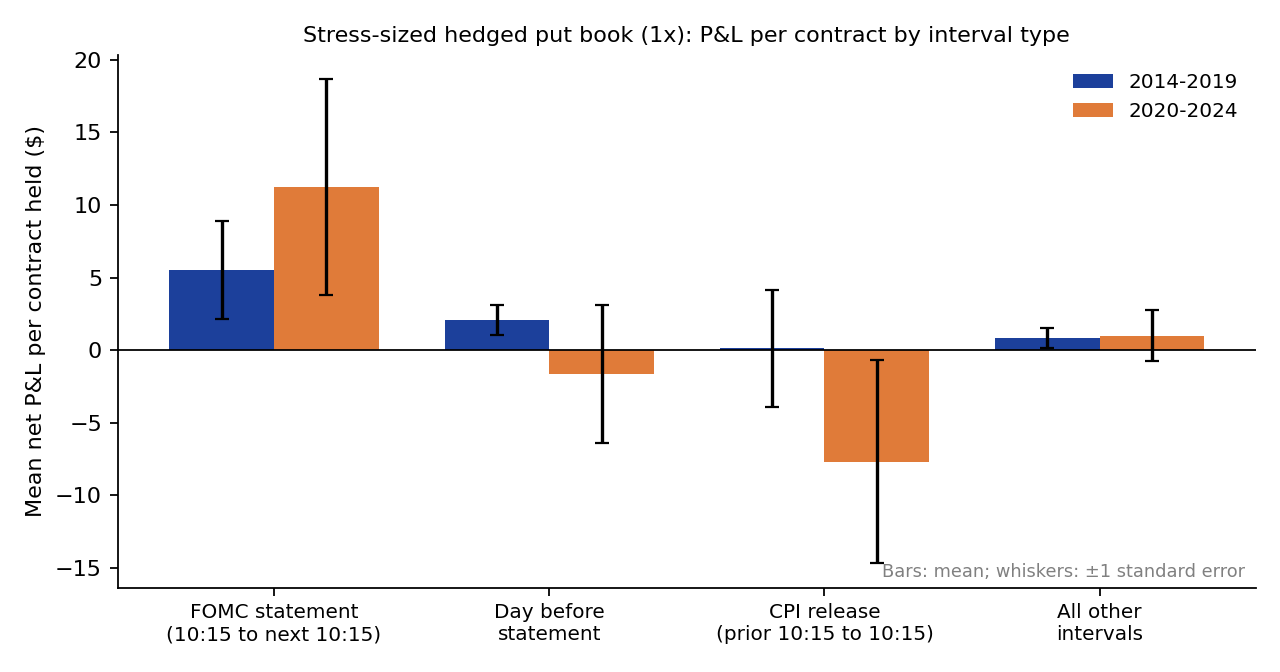
\includegraphics[width=0.92\linewidth]{2026-11-02-fomc-cpi-days.png}\caption{Mean net P\&L per contract held, by interval type and half, hedged book at 1x. Whiskers are \ensuremath{\pm}1 standard error.}\end{figure}

\subsection{How concentrated it is}

\begin{itemize}

\item \textbf{FOMC:} positive in 8 of 11 calendar years. The losing years were 2014 (\ensuremath{-}\$2.6k), 2023 (\ensuremath{-}\$2.8k) and 2015 (about \$0). The five largest intervals, by absolute size, are 25\% of the absolute total.

\item \textbf{CPI:} 2022 (\ensuremath{-}\$9.4k) and 2020 (\ensuremath{-}\$3.0k) make up the loss; 2021 was +\$3.5k.

\begin{itemize}

\item This is the 2022 inflation period, when CPI prints moved the index a lot.

\item It's one regime, not a stable pattern: 2014-2019 CPI intervals average +\$19, t = 0.2.

\end{itemize}

\item \textbf{Unscheduled FOMC actions} are not in the FOMC rows; they fall under ``Other'':

\begin{itemize}

\item \textbf{3 March 2020, 50bp intermeeting cut, 10:00 ET:} the interval ending 10:15 that day lost \$2.1k.

\item \textbf{15 March 2020, Sunday-evening 100bp cut:} the interval from Friday 13 March to Monday 16 March lost \$19.8k, among the book's worst.

\item \textbf{4 October 2019 conference call:} no rate action, so it's not scored.

\end{itemize}

\end{itemize}

\section{What this means for the desk}

These are suggestions; thresholds and structures are the PM's call.

\begin{itemize}

\item \textbf{No card on CPI.} The loss isn't significant and comes from one regime (2022). The obvious rule, skipping entry before CPI, would have fired once in ten years. It couldn't clear any reasonable event floor.

\item \textbf{FOMC is the only lead, and it's weak.}

\begin{itemize}

\item The book already earns the post-statement interval by holding through it.

\item Earning more would mean adding size for the statement interval: for example, a second put opened at 10:15 on statement day and closed the next morning.

\item That pays a round trip each time, and the gain per contract in this book is only about \$7 more than on a normal day.

\end{itemize}

\item \textbf{A possible card, if the PM wants one.}

\begin{itemize}

\item \textbf{Mechanism:} an extra 1x stress-budget slice opened on FOMC statement days and closed at the next 10:15. This needs a small research switch.

\item \textbf{Pass bar,} in the desk's usual form, at 1x and 2x:

\begin{itemize}

\item net P\&L higher than \texttt{hedged} over the full window and in each half;

\item ES 5\% within 1.10\ensuremath{\times} and drawdown within the \$87.5k budget;

\item an event floor of most of the 84 statements.

\end{itemize}

\item \textbf{Expectation:} with only 84 events and a difference that isn't significant against other days, the most likely outcome is a fail at 2x.

\end{itemize}

\item \textbf{Cheaper alternative: shadow mode.} Tag FOMC and CPI days in the live and paper ledger, and revisit with the hold-out years rather than spending trials now.

\end{itemize}

\section{Caveats}

\begin{itemize}

\item \textbf{One mark a day.} Effects inside the day, such as the drift before the announcement or the move between 14:00 and the close, can't be split out. The FOMC interval also includes the next morning.

\item \textbf{Same window as every other test.} This is one more look at 2014-2024. The FOMC mean alone has t = 2.0, but three event types were tested, and the difference from other days is not significant.

\item \textbf{Book P\&L includes the hedge and costs.} Intervals that contain a roll pay the spread whatever the event, though few event intervals do.

\item \textbf{Size varies with IV.} The book holds more contracts when IV is high, so dollar P\&L leans to high-IV years. The per-contract rows correct for this.

\end{itemize}

\section{Sources}

\begin{itemize}

\item Federal Reserve, FOMC historical materials by year, 2014-2020 (meeting dates, including unscheduled and cancelled meetings): \href{https://www.federalreserve.gov/monetarypolicy/fomchistorical2014.htm}{federalreserve.gov/\allowbreak{}monetarypolicy/\allowbreak{}fomchistorical2014.htm} through \href{https://www.federalreserve.gov/monetarypolicy/fomchistorical2020.htm}{fomchistorical2020.htm}.

\item Federal Reserve, FOMC meeting calendars, 2021-2024: \href{https://www.federalreserve.gov/monetarypolicy/fomccalendars.htm}{federalreserve.gov/\allowbreak{}monetarypolicy/\allowbreak{}fomccalendars.htm}.

\item U.S. Bureau of Labor Statistics, Consumer Price Index archived news releases (release dates from the archive's file names): \href{https://www.bls.gov/bls/news-release/cpi.htm}{bls.gov/\allowbreak{}bls/\allowbreak{}news-release/\allowbreak{}cpi.htm}.

\item Desk runs: \texttt{2026-\allowbreak{}10-\allowbreak{}22-\allowbreak{}stress-\allowbreak{}sized-\allowbreak{}puts/\allowbreak{}hedged} (1x, 2x) and \texttt{2026-\allowbreak{}10-\allowbreak{}17-\allowbreak{}always-\allowbreak{}short/\allowbreak{}always25} (1x), from the research registry.

\item Related desk reports: \href{../strategy_research/2026-10-31-signals-beyond-vrp.pdf}{Signals beyond VRP} (FOMC/\allowbreak{}CPI listed as a diagnostic) and \href{2026-10-22-turning-the-backtest-positive.pdf}{Turning the backtest positive}.

\end{itemize}

\end{document}
